\chapter{Problem analysis}
\chlab{problems}

Biomolecular simulations are becoming increasingly important for drug development. In these simulations, force field models are required to describe the interatomic relations of the drug molecules. In order to run a simulation, these force fields require a certain topology, which should include the atom types, bonds, angles, atomic charges and charge group assignments.

%Often used force field models include \verb|AMBER|, \verb|CHARMM|, \verb|GROMACS|, \verb|GROMOS| and \verb|OPLS|. 

\begin{figure}[h!]
\begin{center}
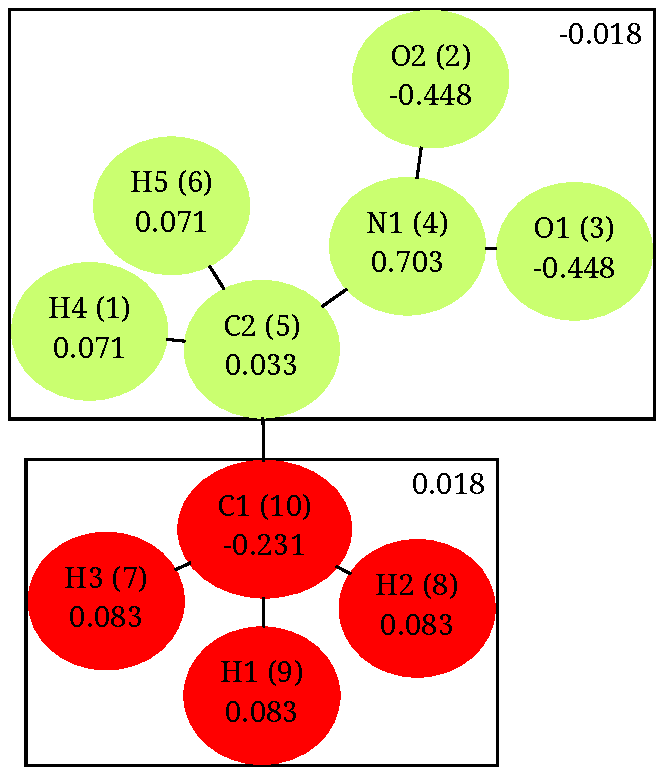
\includegraphics[width=.4\textwidth]{img/partial_charges.pdf}
\caption{Schematic view of nitroethane ($C_{2}H_{5}NO_{2}$), including topology data on atom types, atomic charges and charge groups.}
\figlab{partial_charges}
\end{center}
\end{figure}

\Figref{partial_charges} shows the schematic view of a nitroethane molecule. Here, every oval symbolises an atom. The atom type is the letter on the top rule of the oval, i.e. \verb|H| is the atom type of the sphere \verb|H5 (6)|. The first number indicates the index in the list of atoms of that type (\verb|5| in the example), the second the overall atom index in the molecule (\verb|6| in the example). The bonds between atoms are shown as lines between the ovals and the atomic charges are given by the number at the bottom row of the oval (\verb|0.071| for \verb|H5 (6)|). Finally, the colouring of the atoms and the boxes around them denote a molecular charge group. This is a group of connected atoms, for which the total charge is ideally equal to that of the whole molecule.

In a recent study, El-Kebir, Klau et al. have developed an algorithm that allows for fast and reasonable assignment of charge groups~\cite{canzar2012charge}. As this is now optimised, they currently focus on a different step in the parameterisation: that of calculating the atomic partial charges. Currently, these charges are retrieved using some complex quantum-mechanical calculations. However, as molecules grow bigger, these calculations can take hours or even days to complete. As it is not believed that these calculations can be speeded up, a different approach is needed for finding the partial atomic charges.
% 'Speeded up' is the correct past tense of 'speed up', rather than 'sped up'

One possible way of doing this is by exploiting the similarity of molecules. As similar fragments in molecules often have roughly the same atomic charges, it is possible to retrieve the partial charges of an unparameterised molecule from similar fragments in other molecules for which the charges \emph{are} known. An algorithm for finding these similar fragments is currently being developed at the CWI. However, finding the \emph{best} matches is currently something only experienced chemists can do. A tool is needed that provides them with a view of the unparameterised molecule and the found related fragments. They should then be able to select the best matching fragments, and manually adjust some values if this is really needed.

% TODO: expand
Challenges arise here for the interaction design of the tool. It should be possible to easily compare the related fragments, both with each other and with the unparameterised molecule. How to properly do this is still an open question. As there is currently no software that does this, a proper way of comparing molecule fragments needs to be designed from scratch. This allows for really creating something new, but also creates the challenge of doing it right without any starting point.

Next, the tool should encourage comparing many related fragments in order to find the best match. If, however, there are many related fragments to choose from, the user should be able to easily spot the best ones, as it might otherwise cost too much time to fully parameterise a molecule. This creates another challenge of showing a set of search results in an intuitive way.

Furthermore, as the molecules that will be analysed vary in size from a few atoms to a few hundred, visualisations of the molecules should be given some thought to make sure both large and small molecules look good. This creates yet another challenge, as it is not trivial to show large atoms on a small screen. A good recipe should be developed, such that both small and large molecules will be nicely shown by the tool.

Overall, the biggest challenge is to make the tool work intuitively and make it help to make chemists' work easier, not harder. It should not be the case that, even though they might need to wait a day for their results of the quantum mechanical calculation results, manually parameterising a molecule takes hours. TODO!!
